\subsection{Concurrency in Device Drivers}
\label{bg:concurrency}

Nowadays, multicore machines have become mainstream, allowing operating systems to exploit concurrency for \emph{responsiveness} (latency) or \emph{performance} (throughput). In device drivers, responsiveness is important, because even if there is only a single core, entry points of distinct processes should run concurrently so that no single process hogs the core. Likewise, performance is also important: e.g. network drivers should be able to process incoming packages in a timely manner.

Modern operating systems address the demand for responsiveness and performance by providing multiple sources of concurrency~\cite{corbet2005linux}: a kernel can invoke an arbitrary number of entry points from the same driver concurrently; a running driver process can block and be replaced by another process in the same driver; hardware interrupts can be handled concurrently; delayed code execution is the norm; and the user can insert or remove hardware components without rebooting the kernel (known as hot-plugging). All these possibilities can easily lead to serious concurrency issues, such as \emph{data races}, which can be defined as follows:

\begin{definition}
\label{definition:datarace}
A data race occurs when two distinct threads access a shared memory location, at least one of the accesses modifies the location, at least one of the accesses is non-atomic, and there is no mechanism in place to prevent these accesses from being simultaneous.
\end{definition}

Example~\ref{fig:data_race_example} presents multiple data races that \whoop automatically found in the generic\_nvram Linux char driver (see Section~\ref{evaluation}). The driver can invoke the \texttt{nvram\_llseek} entry point concurrently from two threads $T_1$ and $T_2$, while passing the same \texttt{file} object as a parameter. However, this can lead to multiple possible data races, because $T_1$ and $T_2$ can read/write access the \texttt{f\_pos} field of the \texttt{file} object in arbitrary order resulting into nondeterministic behavior.

\begin{lstlisting}[caption = Data races in the generic\_nvram char driver that \whoop found., label = fig:data_race_example]
static loff_t nvram_llseek(struct file *file,
    loff_t offset, int origin) {
  switch (origin) {
    case 0:
      break;
    case 1:
      offset += file->f_pos; // racy
      break;
    case 2:
      offset += nvram_len;
      break;
    default:
      offset = -1;
  }
  if (offset < 0)
    return -EINVAL;
  file->f_pos = offset; // racy
  return file->f_pos; // racy
}
\end{lstlisting}

The most common technique for eliminating data races is using a \emph{locking} mechanism. Locking a set of program statements that access a shared resource creates a \emph{critical section}, i.e. source code that cannot be executed by more than one thread simultaneously. Example~\ref{fig:lock_example} shows how to use a lock to eliminate the data race in Example~\ref{fig:data_race_example}. The example is tricky, because the return statement can potentially race on the \texttt{f\_pos} field. To fix this issue, we store the result in a temporary variable, inside the critical section.

\begin{lstlisting}[caption = Using a lock to eliminate the data races., label = fig:lock_example]
static loff_t nvram_llseek(struct file *file,
    loff_t offset, int origin) {
  mutex_lock(&nvram_mutex); // lock
  switch (origin) {
    case 0:
      break;
    case 1:
      offset += file->f_pos;
      break;
    case 2:
      offset += nvram_len;
      break;
    default:
      offset = -1;
  }
  if (offset < 0)
    return -EINVAL;
  file->f_pos = offset;
  loff_t res = file->f_pos; // store result
  mutex_unlock(&nvram_mutex); // unlock
  return res;
}
\end{lstlisting}

Lock-based synchronization is a powerful tool for preventing data races in drivers, but careless use of locks has multiple pitfalls~\cite{sutter2005software}. Coarse-grained locking can hurt performance, because it limits the opportunity for concurrency. On the other hand, fine-grained locking can easily lead to deadlocks. Although the Linux kernel provides sophisticated lock-free synchronization mechanisms~\cite{corbet2005linux}, such as atomic read and write operations, in this work we focus on locks. However, we still treat lock-free operations (e.g. atomics) soundly (see Definition~\ref{definition:datarace}), by not regarding them as providing any protection between threads. This is sound but can potentially introduce false positives.

\ADComment{Can we justify the focus on locks a bit more?  E.g., are you able to survey, via grepping, what percentage of Linux drivers make use of locks (likely 100\%?) vs.\ what percentage also make use of lock-free mechanisms?}

\subsection{Reasoning about Thread Interleavings}
\label{bg:happensbefore}

\ADComment{I am unsure as to whether we need this background, but I'm undecided as I'm still getting on top of the rest of the material.}

A fundamental concept in concurrency analysis is Lamport's \emph{happens-before} relation~\cite{lamport1978time}, which denotes a partial-order between all events during the execution of a concurrent program. Happens-before can be defined as follows:

\begin{definition}
\label{definition:datarace}
Let $E_1$ and $E_2$ be two events during a program's concurrent execution. If $E_1$ and $E_2$ are in the same thread and $E_1$ occurs before $E_2$, or if $E_1$ and $E_2$ are in different threads and there is a synchronization mechanism (e.g. locking) that prevents a thread schedule in which $E_2$ occurs before $E_1$, then $E_1 \rightarrow E_2$, where the symbol $\rightarrow$ denotes the happens-before relation.
\end{definition}

Happens-before is transitive, i.e. for any three events $E_1$, $E_2$ and $E_3$, if $E_1 \rightarrow E_2$ and $E_2 \rightarrow E_3$, then $E_1 \rightarrow E_3$. If two events $E_1$ and $E_2$ occur in different threads, and neither $E_1 \rightarrow E_2$, nor $E_2 \rightarrow E_1$ holds, then $E_1$ and $E_2$ happen concurrently, which indicates a data race if the two events access the same shared resource and at least one of the accesses is a modifier.

\begin{figure}[htbp]
\centering
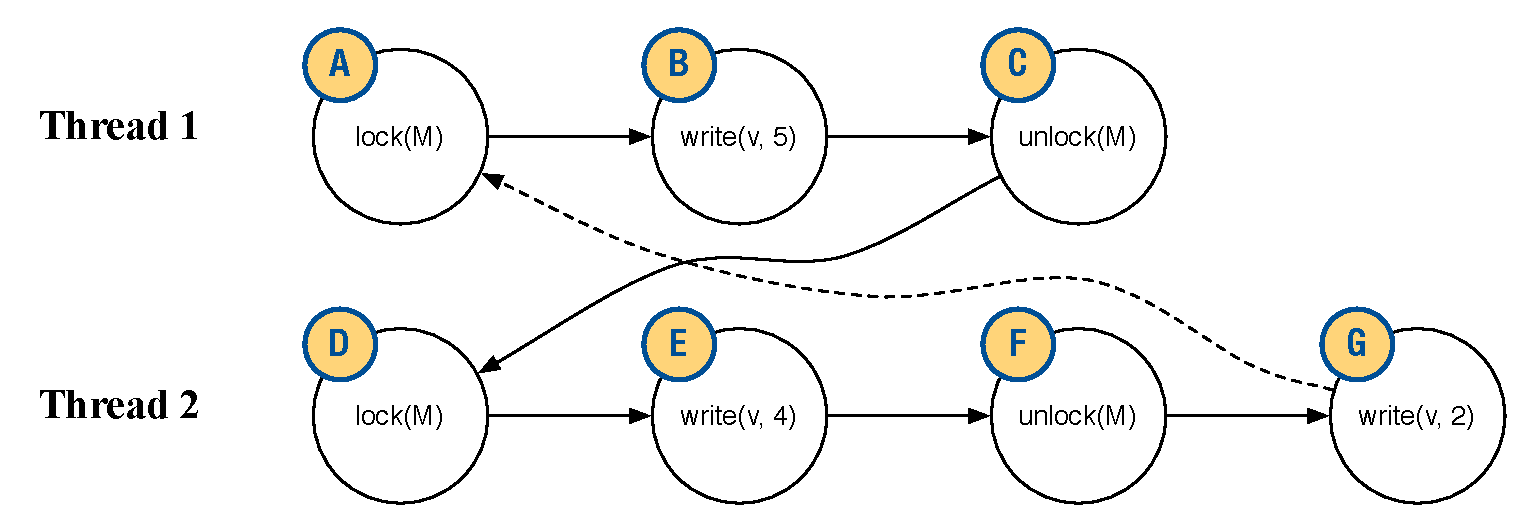
\includegraphics[width=1\linewidth]{img/happens_before.pdf}
\caption{Applying happens-before in two concurrently running threads}
\label{fig:happens_before}
\end{figure}

Figure~\ref{fig:happens_before} shows an example of applying happens-before reasoning in two concurrently running entry points. Each of the three statements $\{A, B, C\}$ in thread 1 is executed before the next one, and thus all of them are ordered by the happens-before relation. The same applies for each of the four statements $\{D, E, F, G\}$ in thread 2. Statement $C$ in thread 1 releases the lock, and subsequently allows $D$ in thread 2 to acquire the same lock. Thus, $C \rightarrow D$. This means that for this specific thread interleaving the set of statements $\{A, B, C\}$ happens before the set of statements $\{D, E, F, G\}$.

The above example also showcases the main limitation of happens-before. If the technique explores \emph{only} this specific thread interleaving, it will miss a potential data race between statements $B$ and $G$, because $B \rightarrow G$ in this specific schedule. Thus, a tool based on happens-before requires a scheduler that produces as many different thread interleavings as possible to increase execution path coverage~\cite{savage1997eraser}. Achieving full coverage with tools based on happens-before is infeasible though, because of the exponential number of possible thread interleavings in realistic concurrent programs. Furthermore, attempting to explore a large number of thread schedules quickly leads to scalability issues~\cite{musuvathi2008finding}, a problem known as state space explosion. Thus, previous work based on happens-before typically explore paths under a certain bound, such as the number of allowed context switches~\cite{qadeer2004kiss}.

\subsection{Reasoning about Locksets}
\label{bg:lockset}

An alternative approach to happens-before, known as \emph{lockset analysis}, resolves around reasoning about the locking behavior of concurrent programs. Lockset analysis was proposed in the context of Eraser~\cite{savage1997eraser}, a dynamic data race detector that tracks the set of locks that \emph{consistently} protect a memory location during program execution. If that lockset ever becomes empty, the analysis reports a potential data race on that memory location. \ADComment{This could be better explained, I think.} This is because an inconsistent lockset suggests that a memory location \emph{may} be accessed simultaneously by two or more threads.

\begin{figure}[htbp]
\centering
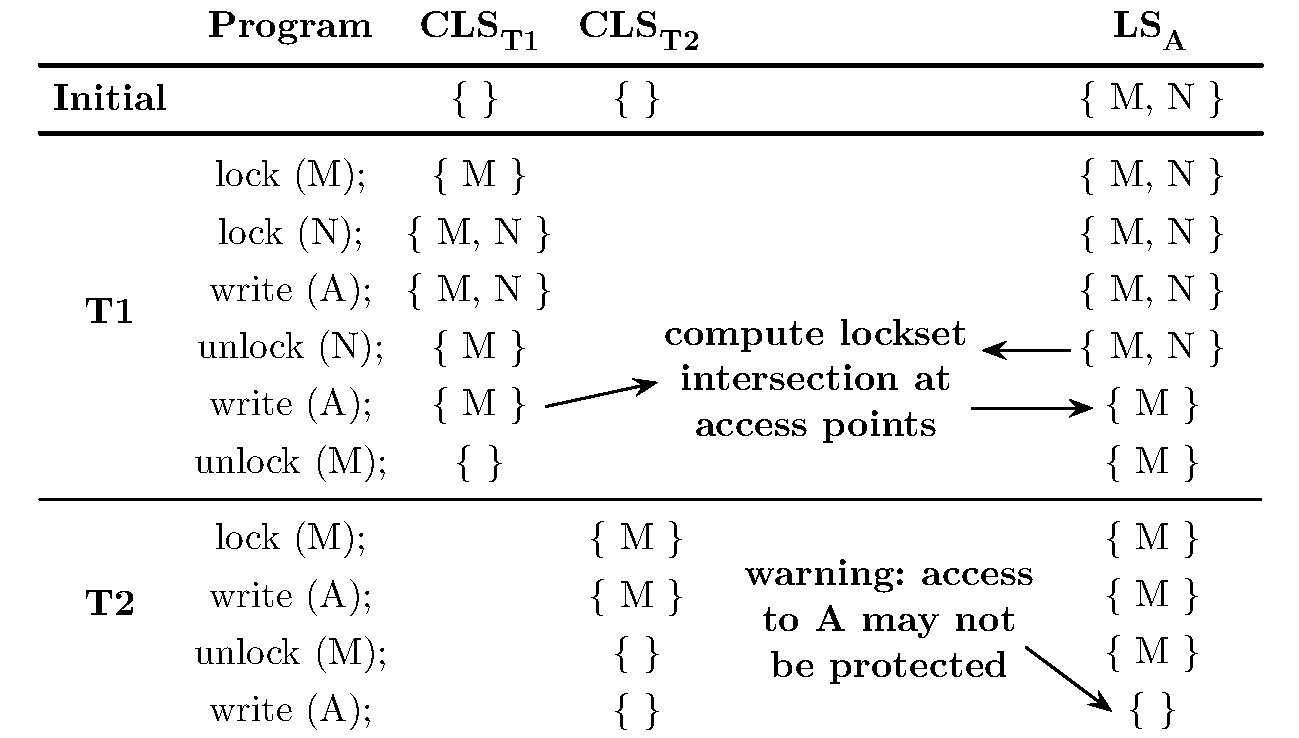
\includegraphics[width=1\linewidth]{img/lockset.pdf}
\caption{Applying lockset analysis on a thread of a concurrent program}
\label{fig:locksets}
\end{figure}

\ADComment{What is missing from the explanation, and from the example you give, is the idea that with a dynamic approach, you run the program and a thread operates in a truly concurrent environment.  You thus only get to see what the thread did on the particular schedule that was followed.  I also think you should use a two-threaded example, instead of a one-threaded example, to show that although thread $T$ might consistently use mutex $M$ to protect variable $A$, this is no good if thread $U$ accesses variable $A$ without holding $M$.}

Lockset analysis for a concurrent program starts by creating a \emph{current} lockset, $\mathit{CLS}_T$, for each thread $T$ of the program, and a lockset, $\mathit{LS}_v$, for each shared variable $v$ used in the program. Initially, $\mathit{CLS}_T$ is empty for every thread $T$, because the threads do not hold any locks on program start. The lockset $\mathit{LS}_v$ for each variable $v$ is initialized to the set of all locks manipulated by the program, because initially each access to $v$ has (vacuously) been protected by every lock. The program is executed as usual (with threads scheduled according to the OS scheduler), except that instrumentation is added to update locksets as follows:
%
\begin{enumerate}
\item After each \emph{lock} and \emph{unlock} operation by $T$, $\mathit{CLS}_T$ is updated to reflect the locks currently held by $T$.
\item When $T$ accesses shared variable $v$, any locks that are not common to $\mathit{LS}_v$ and $\mathit{CLS}_T$ are removed from $\mathit{LS}_v$.
If $\mathit{LS}_v$ becomes empty as a result, a warning is issued that the access to $v$ may be unprotected.
\end{enumerate}

In the example of Figure~\ref{fig:locksets}, we analyze only one thread $T$ and one shared variable $A$ and thus there are two locksets: the current lockset for $T$ ($\mathit{CLS}_T$) and the lockset for $A$ ($\mathit{LS}_A$).

Figure~\ref{fig:locksets} shows an example of applying lockset analysis on a concurrent program consisting of two threads $T_1$ and $T_2$, both accessing the shared variable $A$. Thus, we have to analyze three locksets: the current locksets $\mathit{CLS}_1$ and $\mathit{CLS}_2$ for $T_1$ and $T_2$ respectively; and the lockset $\mathit{LS}_A$ for $A$.

\ADComment{I folded some of the discussion of the example into the above more general description of locksets.  Assuming you do produce a two-threaded example, please put in a brief explanation of it.}

In contrast to analyses based on happens-before, lockset analysis has the potential to scale well, because it does not need to reason about all possible thread interleavings to achieve good code coverage. The technique, though, suffers from imprecision (i.e. can report false bugs), because a violation of the locking discipline does not always correspond to a real data race~\cite{savage1997eraser, pozniansky2003efficient, o2003hybrid, elmas2007goldilocks, flanagan2009fasttrack}. Furthermore, code coverage in dynamic lockset analysis tools, such as Eraser, is limited by the number of explored execution paths. To counter these limitations, some techniques~\cite{pratikakis2006locksmith, voung2007relay} have explored the idea of applying lockset analysis in a static context, using dataflow analysis. In this paper, we also present a static lockset analysis method that involves generating verification conditions to be discharged to a theorem prover.
